\chapter{Implementácia prostredia}
Prostredie bolo implementované v jazyku C++ vzhľadom na použité nástroje Flex a Bison. Kapitola je zameraná na použité štruktúry, vysvetlenie výberu týchto štruktúr a použité algoritmy. Pre potreby vysvetlenia implementácie sa používajú nasledujúce pojmy:
\begin{description}
\item[Kontext]\hfill \\
	Pojem kontext je v tejto kapitole používaný sa definovanie relevantých okolností, za akých je vykonávaná inštrukcia kódu. Zjednodušene povedané ide tú najkratšiu možnu postupnosť inštrukcíí pred volaním danej inštrukcie. Významné sú iba volania funkcií a definovanie nových blokov. Matematicky povedané, kontext je usporiadaný zoznam volaní funkcií a definovaní nových blokov. Uvažujme kód v tabuľke \ref{tab:rek}, potom kontext inštrukcie na riadku 3 je $<main(),f(),\{>$. Napriek tomu, že funkcia f je rekurzívna a hĺbka zanorenia môže byť iná. Z opačného pohľadu, v rovnakom kontexte sa môžu vyskytovať viaceré inštrukcie. V našom príklade je tomu tak pri volaní funkcie f na riadku 4. kontext volania  funkcie f na riadku 9 je $<main()>$.
\item[Premenná] \hfill \\
	Pojem premenná reprezentuje dáta pomenované jednoznačným reťazcom začínajúcim písmenom alebo podtržítkom. Napríklad \emph{integer test} je premenná s názvom test, ktorá je typu integer. Slovo test by v danom kontexte nemalo byť použité pre inú premennú. V tabuľke \ref{tab:rek} je teda premenná \emph{a} zadefinovaná chybne, pretože existujú dve premenné \emph{a} v rovnakom kontexte.
\item[Premenné robota]\hfill \\
Premenná robota je taká premenná, o ktorej robot predpokladá, že data v nej sa menia len v závislosti na jeho akciách. Predpokladajme, že v tabuľke \ref{tab:rek} je definovaný kód robota A. Potom a je premenná robota A. Pokiaľ existuje iný robot B, nemá žiaden vplyv na premennú a robota A.
\item [Tick] \hfill \\
	Označuje je jednotka virtuálneho času sveta. Počet tikov, koľko trvá jedno kolo, je záväznú pre všetkých robotov a závisí na plánovači. Defaulte sa jeden tick rovná jedno kolo.
\item[Penalizácia za inštrukciu]
	Je počet tikov, ktoré robot potrebuje na vykonanie inštrukcie. Pre rôzne inštrukcie môže byť (a typicky bude)rôzna.
\item [Program robota]
	Značí postupnosť inštrukcií.
\item [ProgramPointer]
 	Je ukazateľ na inštrukciu v programe. Druhy inštrukcií a ich vplyv na svet je popísaný v tabuľke \ref{tab:instrukcie}.
\item[Cieľ určenia]
	Tento pojem reprezentuje políčko na mape sveta, kam sa má robot dostať. Teda cieľ určenia je oblasť definovaná pomocou kódových slov \emph{VisitSeq} alebo \emph{Visit}.
\end{description}

\begin{table}
\centering
\begin{tabular}{| lll |}
\hline
1&void function f()&\\
2&\{&\\
3&&integer a;\\
4&&f();\\
5&&integer a;\\
6&\}&\\
7&int main()&\\
8&\{&\\
9&&	f();\\
10&\}&\\
\hline
\end{tabular}
\caption{ Príklad kódu robota }
\label{tab:rek}
\end{table}

%Samotná hra prebieha tak, že roboti vykonávajú užívateľom definovaný kód až do okamžiku, keď dosiahnu víťazný stav alebo kým nezostane na bojisku maximálne jeden robot. Cieľ môže byť pre každého robota rozdielny a je jeho súčasťou. Hra nie je zabezpečená proti nekonečne dlhotrvajúcim cyklom (napríklad keď každý robot stojí na mieste), predpokladá sa v tomto prípade vstup od uživateľa, ktorým hru preruší.

\section{Implementácia jazyka}
Každý robot má vlastný program, hráčom definovaný, podľa ktorého sa správa. Tento program sa zo strany robota skladá z postupnosti základných inštrukcií, ktoré sú ďalej nedeliteľné. \\ 
Najskôr bolo nutné určiť si základnú štruktúru práce s inštrukciami a premennými. Základným problémom bolo uchovávanie premenných a ich neskoršie spracovanie. Keďže premenné sú definované jednoznačným identifikátorom. Vhodnou je štruktúra, ktorá vyhľadáva podla reťazca. Ako mapa názvov premenných bola uvažovaná štruktúra podľa \cite{trees}
\subsection {Burst tree} 
Burst tree je stromová štruktúra, ktorá bola špeciálne vyvinutá pre rýchly prístup k záznamom podľa textového kľúča.\\
Princíp burst tree je jednoduchý. Strom pozostáva z dvoch úrovní. Posledná vrstva sú kontainery. Tie obsahujú jednotlivé záznamy, ktoré chceme vyhľadávať podľa textového kľúča. Záznamy v kontajneri sú usporiadané buď do obyčajného binárneho stromu, alebo do akéhokoľvek iného zoznamu. Vrstva nad kontajnermi je prefixový strom. Prefixový strom pozostáva z uzlov, ktoré obsahujú prefix vložených textových reťazcov. S hĺbkou stromu sa zvyšuje dĺžka prefixu. List tohoto prefixového stromu bude obsahovať kontajner. Algoritmus vyhľadania záznamu v tejto štruktúre je nasledovný, ako je popísaná \cite{trees}:\\ 
\begin{enumerate}
\item Najskôr je uvažovaný uzol koreňom stromu a počiatočná hĺbka je 0.
\item Prefixový strom je prechádzaný od koreňa.
\item Ak je hĺbka väčsia ako reťazec, potom sa záznam pridá do aktuálneho uzla, kam sa už dostal, pod prázdnym znakom.
\item Pokiaľ sa nenájde zodpovedajíci prefix alebo hĺbka hľadania presiahne hĺbku stromu, algoritmus skončí s nenájdeným reťazcom.
\item Pokiaľ sa našiel zodpovedajúci prefix v danej hĺbke, aktuálny uzol sa zmení na tento uzol a prechádajú sa jeho potomkovia.
\item Potomok uzlu môže byt opäť prefixový strom alebo kontajner.
\item Ak je potom kontajner, potom sa prechádza ten, algoritmom zodpovedajúcim štruktúre v kontajneru
\end{enumerate}
Algoritmus vkladania je však ten, vďaka ktorému získala štruktúra meno:\\
\begin{enumerate}
\item Pomocou vyhľadávacieho algoritmu je nájdený kontajner, kde patrí záznam.
\item Ak nie je kontainer dostatočne naplnený, potom sa záznam pridá do kontajneru a algoritmus skončí.
\item Ak je dostatočne naplnený, potom nastáva burst fáza algoritmu
\begin{itemize}
\item Vytvorí sa nový uzol prefixového stromu.
\item Uzol sa zaradí to prefixového stromu namiesto kontajneru
\item Všetky záznamy z pôvodného kontajneru sa zaradia do kontajnerov nového uzlu
\item Je nutné opakovať, až pokiaľ nie je splnená podmienka pre burst fázu
\end{itemize}
\end{enumerate}
Názvy premenných je nutné rozlišovať vzhľadom na kontext. Kontext bol do tejto štruktúry zapracovaná následovne: K menu každej premennej sa pridá názov funkcie, v ktorej bola premená deklarovaná. Tým sa dosiahne jej unikátne meno. Problém v počte deklarovaných blokov sa vyriešil pomocou ďalšej premennej, ktorá signalizovala hĺbku v ktorej bola premenná definovaná. Pokiaľ sa vyskytla deklarácia, táto premenná sa nastaví a aktívnu v danej hĺbke. V okamihu opustenia bloku sa všetky premenné zmenili na neaktívne. \\
Štruktúra Burst tree sa neskôr ukázala ako bezvýznamná, keďže sa k nej pristupuje len vo fázi inicializácie a tam nie je potrebné štruktúru optimalizovať. Princíp ukladania názvov premenných a štruktúra ukladania ale napriek tomu zostali. \\
\subsection{Štruktúra vykonávania inštrukcií}
Pre pochopenie práce inštrukcií a spôsob, akým menia mapu, je nutné si definovať pojmy:
\begin{description}
\item [Stav robota]
	Stav robota vzhľadom na svet charakterizuje štvorica: (InstructionPointer IP, Hitpoints HP, FieldOfSight fs, Direction direct), kde 
\begin{itemize}
\item InstructionPointer je odkaz do štruktúry programu robota hovoriaci, ktorá inštrukcia je na rade
\item HP je nezáporné celé číslo popisujúce životnosť robota
\item FieldOfSight je štruktúra obsahujúca objekty v zornom poli od posledného volania funkcie \emph{see()}, volanej bez parametrov 
\end{itemize}
\item[Stav robota] \hfill \\
	Stav robota s ohľadom na inštrukcie, ktore vykonáva, charakterizuje (PointerStack PS, ValueStack VS, Memory m) kde
\begin{itemize}
\item PS zoznam pointerov do štruktúry programu
\item VS je zásobník všetkých naloadovaných hodnôt, parametrov  a návratových adries z funkcií. Značí sa $[values|rest]$, kde values je prvý prvok na spracovanie ( takže posledný pridaný ). Zmena zásobníku ude značená $ oldValues -> newValues $
\item Memory je štruktúra pre prideľovanie miest na zápis dát
\end{itemize}
\label{StavRobota}
\item[Svet] \hfill \\
Na svet sa dá matematicky popísať ako dvojica $< RobotsList, Map >$, kde:
\begin{itemize}
\item RobotsList je cyklický zoznam robotov s programami. Ich telo by sa v tomto okamihu malo nachádzať na mape. Roboty v tomto zozname sa počas priebehu boja nemenia. V okamihu, keď umrú, sa ich telo kvôli zobrazovaniu stále ocitá v mape. Jediné, čím sa prejaví ich smrť je, že plánovač sa nikdy nedostane do stavu ''pripravený'', takže interakcia tohoto robota s mapou bude nulová.
\item Map reprezentuje mapu, v ktorej sa roboti pohybujú. Na mape môžu pribúdať alebo miznúť objekty. Pribúdanie objektov súvisí s vystrelením zbrane, odoberanie môže nastať v okamihu, keď sa podarí zničit stenu alebo eliminovať strelu.
\end{itemize}
\end{description}
Vygenerované inštrukcie sa nachádzajú u robota v jednom veľkom poli, vrátane inštrukcií všetkých funkcií. K inštrukciám ale existuje pomocná trieda Core, ktorá obsahuje deklaráciu všetkých funkcií vrátane ich parametrov, ukazovateľom na robotovo telo a ProgramCounterov pre zistenie, ktorá inštrukcia sa má vykonať. \\
Pre všetky nasledujúce inštrukcie, ktorých vykonanie sa priamo prejaví na mape. Predpokladajme, že svet je v stave $<RobotsList, Map>$, kde RobotsList je postupnosť objektov $(robot1,robot2, robot3,...,robotN)$ a Map je dvojrozmerná matica obsahujúca objekty a informácie o nich. Inštrukcie vizuálne meniace mapu:\\
move:\begin {itemize}
\item Svet:$ < RobotsList, m) > $
\item Bot: $ < NewIP, Hp, direct> $
\end {itemize}
turnLeft, turnRight \begin{itemize}
\item $Svet:  <RobotsList, m>$
\item $Bot:  < NewIP, Hp, NewDirect)>$
\end{itemize}
turn  \begin{itemize}
\item $Svet:  < RobotsList, m > $
\item $Bot:   < NewIP, Hp, NewDirect)> $
\end {itemize}
see  \begin{itemize}
\item $Svet:  <RobotsList,m> $
\item $ Bot:  < NewIP, Hp, NewDirect)> $
\end {itemize}
shoot \begin {itemize}
\item $ Svet:  < RobotsList, m.insert(strela)> $ 
\item $ Bot:  < NewIP, Hp, Direct)>  $
\end {itemize}
\indent
kde NewIP je tu nový ukazateľ do programu robota, nutne odlišný od predošlého. NewDirect je číslo 1-4 označujúce aktuálne natočenie robota.
Reinsert je funkcia, ktorá vloží na miesto blízko robota strely v definovamom smere. Ošetrovanie kolízií pri pohybe je už záležitosťou mapy. Preto sa Hp zdá byť pri vykonávaní inštrukcií statické, jeho zníženie ale je možné až pri kontrole kolízií.

Ďalšie inštrukcie nemajú vplyv na svet, preto sú uvedené oddelene. Tieto inštrukcie robot vykonáva počas svojho premýšľania. Vykoná ich toľko, dokedy bude lánovač pripravený. Pri týchto inštrukciách robot potrebuje poznať len svoje premenné. Po prevedení takýchto inštrukcií sa mení stav robota podľa tabuľky \ref{VnutroBota},kde
\begin{itemize}
\item IP+1 znamená posun v aktuálneho pointera v programe robota o jednu inštrukciu ďalej
\item newIP je uloženie aktuálneho pointera na inštrukciu a vyhlásenie iného pointera za aktuálny (typicky začiatok procedúry alebo funkcie), informácie o tom, ktorý ProgramPointer je aktuálny, sa získajú pomocou triedy Core. Tá tým vlastne reprezentuje mozog robota.
\item newMemory je pamäť robota po obsadení/uvoľení príslušného miesta.
\item memory.deleteTemp() je označenie poslednej premennej alokovanej v pamäti za neplatnú a teda uvoľnenie miesta v pamäti.
\item memory.temp() je uloženie výsledku aritmetických operácií na ValueStack. Miesto pre zápis takejto anonymnej premennej sa získa z pamäti robota pri požiadavke o anonymnú premennú.
\item DeleteIP je zrušenie aktuálneho pointera na funkciu a obnovenie predchádzajúceho na inštrukciu, pred ktorou bol prerušený. 
Na rozdiel od \ref{tab:instrukcie} sú inštrukcie popísané vzhľadom na skupinu, ku ktorej patria a táto tabuľka obsahuje detailnejší popis.
\end{itemize}

\begin{table}[ht]
\centering
\caption{Vnútorné príkazy robota}
\begin{tabular}{|l|c|}
\hline\hline
Inštrukcia & Stav robota po inštrukcii \\
\hline
create & $ IP+1, [rest]->[rest], newMemory$ \\
store & $ IP+1, [a,b|rest]->[rest], memory$ \\
aritmetické operácie & $IP+1, [a,b|rest]->[m.temp()|, newMemory$ \\
relačne operácie & $IP+1, [a,b|rest]->[m.temp()|rest], newMemory$ \\
call &  $ newIP, [rest]->[rest], newMemory$\\
startBlock & $IP+1, [rest]->[rest], memory$\\
endBlock & $IP+1, [rest]->[rest], newMemory$\\
removeTemp & $IP+1, [rest]->[rest], memory.deleteTemp()$\\
load & $ IP+1, [rest]->[a|rest], memory$\\
duplicate & $ IP+1, [a|rest]->[a,a|rest], memory$\\
restore & $ DeleteIP, [rest]->[returnValue|rest], newMemory$\\
pop & $ IP+1, [a|rest]->[rest], memory$\\
\hline
\end{tabular}
\label{VnutroBota}
\end{table}
\subsection{Zaujímave nastavenia a efekty}

Velmi špeciálny je prípad, keď užívateľ nenastaví robotovi žiadnu pamäť. Takýto robot nie je schopný si zapamätať jedinú premennú a ani vraciať návratové hodnoty. V algoritme by nemali byť definované žiadne funkcie, ale iba procedúry, kedže funkcie a procedúry nezaberajú robotovi pamať. Teda v tomto prípade môže dojsť k masívnemu využitiu rekurzií. Samotne vstavané príkazy sú však vlastne funkcie, ale kedže sa nikam nemajú priradiť, ich návratová hodnota sa zahodí. Nevýhodou tohoto typu bota je však skutočnost, že strieľať alebo pohybovať sa môže len pomocou konštanty. Iné hodnoty nemajú garantované miesto v pamäti.

\subsection{Zrak robota}

\begin{figure}
\centering
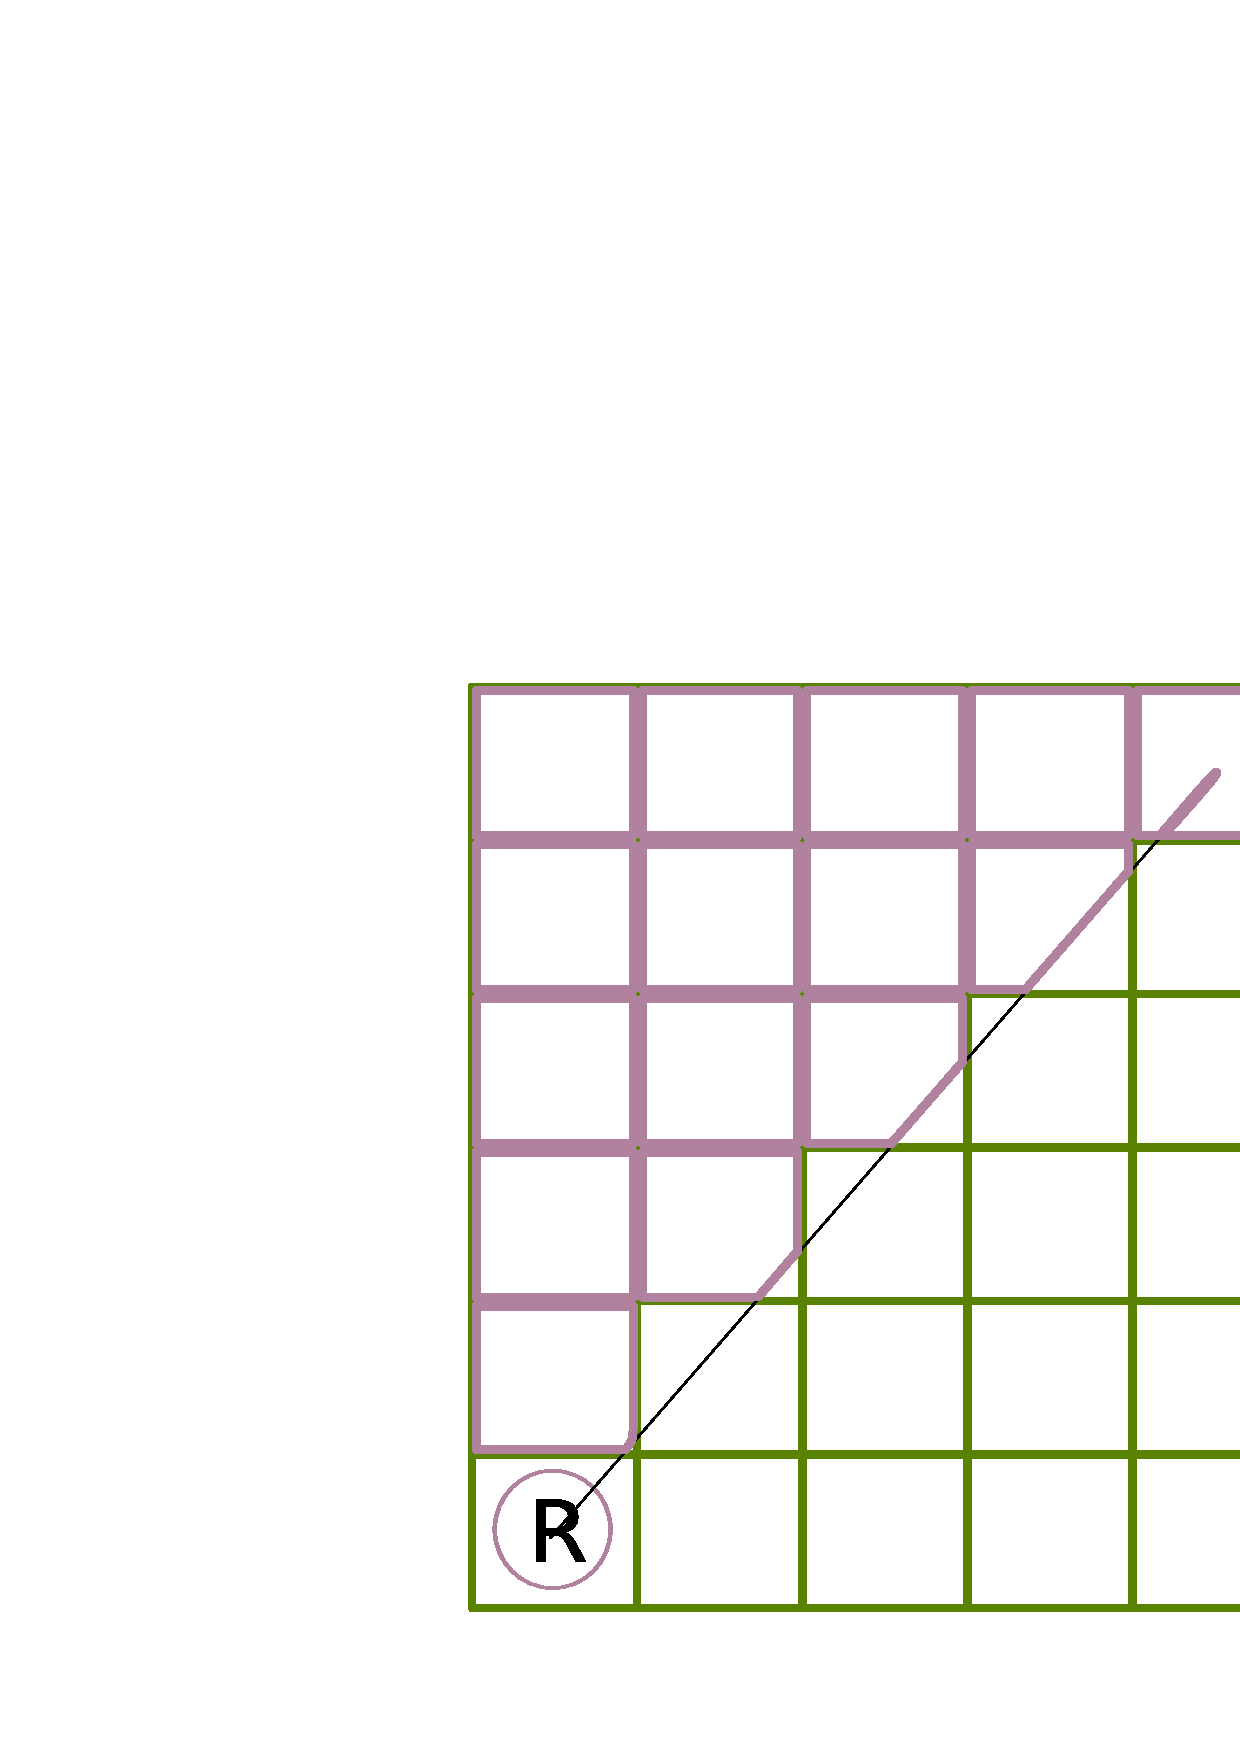
\includegraphics[totalheight=0.2\textheight,width=.6\textwidth]{chooseVisible}
\caption {Výber parametrov pre zrak robota}
\label{choosing}
\end{figure}

\begin{description}
\item[Zorné pole robota]\hfill \\
Pod zorným poľom robota rozumieme hornú polovicu trojuholníka určeného uhlopriečkou medzi vrcholmi obdĺžnika o veľkosti X,Y, kde, X, Y sú odvesny pravouhléhotrojuholníka s preponou rovnou viditeľnosti mapy. \\
Robot vidí objekt v okamihu, keď vidí stred políčka, na ktorom objekt stojí a úsečka spájajúca tieto dva body nepretína žiadny ďalší blokujúci objekt. Blokujúci objekt je definovaný implementáciou, v našom prípade je blokujúci objekt robot a stena, neblokujúci strela. Toto rozdelenie vychádza z bežneho pozorovania, že drobná strela nemá tendenciu zakrývať výhľad.
\end{description}
Vo vstupe si užívateľ má možnosť nastavit premennú, ktorá ovplyvňuje to, ako ďaleko bude robot vidieť do strán. Je to premenná $\alpha$, ktorá označuje uhol, pod ktorým vidí robot na jedno oko. Pochopiteľne má robot symetrické oči a teda do druhej strany vidí pod rovnakým uhlom. Jedným z pomerne rýchlych spôsobov, ako určiť viditeľné objekty, je algoritmus rozďeľujúci obdĺžnik zorného poľa na niekoľko rovnakých častí.
Obdĺžnik môže mať vzhľadom na implementáciu maximálne obsah 32, čo je na väčšine architektúr veľkosť integeru. Samotné detekovanie toho, čo robot vidí, prebieha nasledujúco: \\
\begin{figure}
\centering
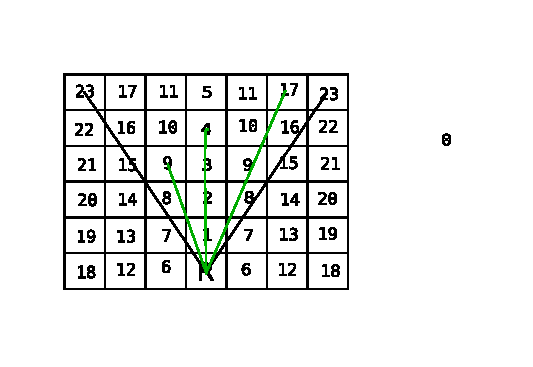
\includegraphics[totalheight=0.4\textheight,width=.8\textwidth]{visibility}
\caption {Viditeľnosť robota s parametrom uhla $20^\circ$}
\label{fig:visibility}
\end{figure}
Nech má obdĺžnik rozmery (x,y) a jeho dolný ľavý vrchol je na pozícií (0,0), čo je v podstate pozícia bota. Obdĺžnik je teda rozdelený na XxY menších obdĺžničkov. Každý z nich má svoje poradové číslo a masku, ktorá má na i-tej pozícií jednotku práve vtedy, ak úsečka začínajúca v bode [0.5,0.5],čo je stred políčko s robotom, a stredom skúmaného políčka prechádza políčkom s identifikaćným číslom ID. Takto ale robot bude vidieť len na jednu stranu, ale keďže druhá polovička je presne symetrická, môžeme tieto práve vygenerované masky použiť, viď \ref{visibility}  na obe strany bez upravovania. \\
Podľa obrázka \ref{fig:visibility} bude mať políčko s ID 4 masku 1111, pretože na to, aby ho bolo vidieť, je nutné vidieť políčka s ID 1,2,3. Podobne políčko 9 bude mať masku 110000011, pretože úsečka spájajúca tieto dva body prebieha tiež týmito políčkami. Zistenie, či práve toto políčko je pretnuté úsečkou, sa takto zjednodušuje na nájdenie všeobecnej rovnice priamky s koncovými bodmi v stredoch týchto dvoch políčok. Zistenie, či pravý dolný vrchol a ľavý horný vrchol patria rovnakej polrovine generovanej touto priamkou.\\
Za života robota sa jeho zrak nemení a teda môžeme použiť tieto vygenerované masky bez ďalšieho prepočítavania. Pri volaní metody see(), ktorá dodá viditeľné objekty robotovi, potom stačí namapovať náš obdĺžnik na príslušné miesto na mape(podľa robotovej pozície a natočenia), nastaviť 1 na i-té miesto políčka s ID = i, na ktorom nie je nič alebo len neblokujúci objekt, a výslednú masku porovnať s predtým vypočítanou maskou každého políčka, na ktoré by robot mohol vidieť. Nech zisťujeme, či vidíme objekt na pozícií na mape X,Y, ktorý sme namapovali na políčko s ID = I a maskou M. Ak výsledná maska má jedničky presne na tých istých miestach ako M, potom I je viditeľné, pretože všetky políčka, na ktorých I záviselo, boli označené ako viditeľné. \\
Nech existuje také políčko s ID = P, na ktorom je nejaký blokujúci objekt. Potom vo výslednej maske bude na P-tom mieste 0 a políčko I, ak úsečka spájajúca stredy políčok robota a I prechádzala cez P, bude mať na P-tom mieste 1. Maska políčka I bude mať teda o minimálne jednu 1 viac ako výsledná maska a teda políčko bude označené ako neviditeľné.\\
Na obrázku \ref{fig:visibleo} je červeným znázornený objekt, ktorý robot už neuvidí a zelenou, ktorý naopak uvidí. Napríklad robot R je viditeľný, pretože pred ním je strela S a keďže je neblokujúca, políčko 4 pripojilo na výslednej maske 1 na 4.pozícií. Pozícia 5 má masku 1111 a teda je viditeľná.
\begin{figure}
\centering
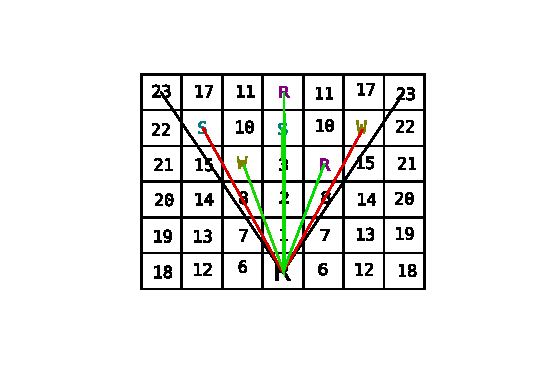
\includegraphics[totalheight=0.4\textheight,width=.8\textwidth]{VisibleObjects}
\caption { Objekty v zornom poli robota}
\label{fig:visibleo}
\end{figure}
\indent
\newline
\indent Tento spôsob má ale nevýhodu pri použití v programoch typu Codewars. Predpokladá totiž, že v okamihu žiadosti o naplnenie viditeľných objektov budú tieto objekty stáť presne v strede daných políčok, resp. že bojisko bude rozškatuľkované. Ak by povedzme jedna stena stála presne nedzi dvoma políčkami, už nie jasné, aké políčka robot vidí. Preto bol primo v implementácií použitý spôsob porovnania uhlov viditeľnosti.
\\
\begin{figure}
\centering
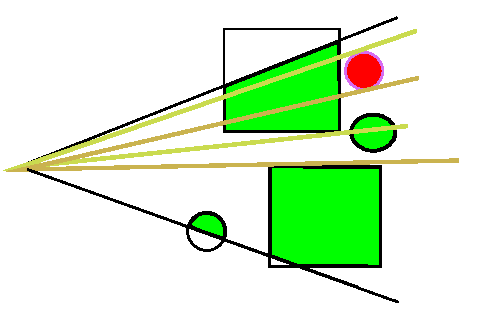
\includegraphics{visibility2}
\caption { Objekty v zornom poli robota podľa fruhého algortimtmu. Červeným je vyznačený objekt, ktorý nie je vidno.}
\label{fig:visibleo}
\end{figure}
\indent
\section{Priebeh penalizácie za inštrukciu}
Nech je na rade robot R. R sa pozrie, či už ubehla dostatočne dlhá doba od vykonania jeho poslednej akcie. Ak áno, R začne vykonávať inštrukciu, na ktorú práve ukazuje jeho ProgramPointer. Po vykonaní tejto inštrukcie si poznamená, koľko ho stála tickov. Ak ešte neprebehla dostatočne dlhá doba, potom počká a na rade je ďalší objekt. Penalizácia prebieha podľa aktuálnej tabuľky penalizácií, ako bola nastavená v základnom menu. \\

Týmto spôsobom sa efektívne vyrieši prípad, keby robot premýšľal príliš dlho, alebo keby sa zacyklil. Keďze po každej vykonanej inštrukcii predá riadenie daľšiemu objektu, zacyklenie sa pozná len podľa toho, že robot sa nebude hýbať, ale nijak to nespomalí ostatné objekty.%TODO ref
\newline
Nech je na rade objekt rôzny of typu 'robot'. Potom tento objekt má konštantnú penalizáciu (strela štandartne 0) a jeho program obsahuje iba inštrukcie, ktoré interagujú s bojiskom. Sú rôzne v závislosti na type objektu.

\subsection{Možné plánovače}

Rozhodovanie robota, či má vykonať inštrukciu, prebieha pomocou plánovača. Problémom je určiť, kedy je plánovač pripravený vzhľadom na penalizácie za inštrukciu. Veľkosť penalizácií sa dá použiť dvoma spôsobmi:
\begin{enumerate}
\item Jedna inštrukcia trvá toľko kôl, koľko je jej penalizácia. Táto konštrukcia zodpovedá kontinuálnej dlhodobej práci ( predstave, že CreateVariable skutočne nejakú premennú vytvára a teda koná prácu ).
\item Opačný prístup. Plánovač dostane do vienka nejaký čas a snaží sa ho čo najviac využiť, vyplniť inštrukciami.
\end{enumerate}
Prvý prístup je pomerne priamočiary, ľahko implementovateľný  na radu sa pomerne rýchlo dostanú aj ďalši roboti. Jeho nevýhodou je, že pokiaľ čaká, nemôže reagovať na ďalšie veci. Keby napríklad inštrukcia see stála 5 kôl, robot inštrukciu vykoná a čaká 5 kôl. Medzičasom sa mu zorné pole naplní informáciou, že videl strelu.  Rýchlosť strely je ale pomerne vysoká a preto je možné, že keď plánovač bude zase pripravený, strela bude preč a teda mimo zorného poľa robota. Robot tak nemôže určiť polohu, smer, pohyb, atď.\\
Druhý spôsob sa k inštrukciám správa ako závislým na čase. Penalizácie nebudú značiť priamo čas, ale akú časť z pevne daného množstva F zaberajú. Predpokladajme, že prešlo X kôl. Plánovač, implementovaný podľa druhého algoritmu, bude naviac obsahovať nezáporné číslo, ktoré zostalo pri poslednom vykonaní inštrukcie. Nasledujúca inštrukcia mala totiž väčšiu penalizáciu ako počet bodov, ktorý zostal. K tomuto nezápornému číslu sa pridá naše pevne dané množstvo F. V okamihu, keď je čas menší ako penalizácia inštrukcie, sa plánovač stane nepripravený, inak zostáva v stave pripravený. Pseudokód pre tento spósob je popísaný v tabuľke \ref{tab:sched2}\\
Tento spôsob je viac šetrnejší k robotovi, z pohľadu robota sa zastaví po čas. Požas tohoto zastaveniamôže reagovať a objekty.\\
\begin {table}
\centering
\begin{tabular}{|ll|}
\hline
Uint32 diff= actualTime - timeLastUpdate; &\\
while (diff $>$ 0)&\\
\{& \\ 
&diff-=nextInstruction.penalize();\\
&nextInstruction.run();\\
&Pointer ++; \\
\}&\\ 
\hline
\end{tabular}
\caption{Pseudokód plánovača druhého typu}
\label{tab:sched2}
\end{table}

\section{Hracia plocha} % z coho sa sklada
Na začiatku hry sa vygeneruje mapa s veľkosťou, ktorú zadá užívateľ, alebo sa načíta už uložená mapa. Pozostáva zo voľných políčok a stien. Steny sú rôzneho typu, viď \ref{walls}. Pre vyššiu užívateľskú prívetivosť bol implementovaný generátor mapy. Generuje ''kostru'' mapy, teda pridáva iba základné steny.
\subsection{Generovanie map}% ako sa generuje, podpora ukladania, zadne zhluky, vyhody, nevyhody, 
iNa vygenerovanie máp sa osvedčil jednoduchý ''pažravý'' (greedy) algortimus. Celá mapa sa rozdelila na množstvo malých kúskov, ktoré predstavovali ''potravu''. Do takéhoto prichystaného prostredia bol vypustený ''had'', jednoduchá entita s primárnym cieľom čo ajviac sa nažrať. Had mal sprvu náhodný algoritmus. Tkto vygenerovaná mapa bola tvorená jedným pomerne malým zhlukom. Preto bol k hadovi pridaný mechanizmus, ktorý ho 'ťahá' na tú strane, ktorá je najvzialenejšia. Mapy, vygenerované pomocou tohto algoritmu vyplňovali mapu ďaleko viac. Problém bol, že cesty v mape vzniknutej týmto spôsobom boli veľmi úzke. Preto ďalšie vylepšenie zahrňovalo vytvorenie ďalších hadov, takzvaných potomkov. Títo sa veľmi pravdepodobne nenarodili na rovnakom mieste ako ich rodič, preto ich túžba vydať sa iným zmerom bola rozdielna. Takto spustený algoritmus mal pomerne dobré výsledky až na časti, keď išli hadi cestou sami. Preto bola pridaná možnosť, že had počas žrania bude tlsnúť. Tým sa vytvoria pre robotov koridory. Po vyskúšaní viacerých modifikácií, kedy sa majú hadi množiť a kedy tlstnúť, sa osvedčilo zadať 25\% šanciu na tlstnutie a náhodný algoritmus na rozmnožovanie. Algoritmus je pomerne rýchly a výstupom sú mapy, ktoré sú pre robota dostatocne široké a pritom rozľahlé ( cez celú mapu ), viz obrázok \ref{fig:mapa} pre veľkosť mapy 1000x1000.
\begin{figure}
\centering
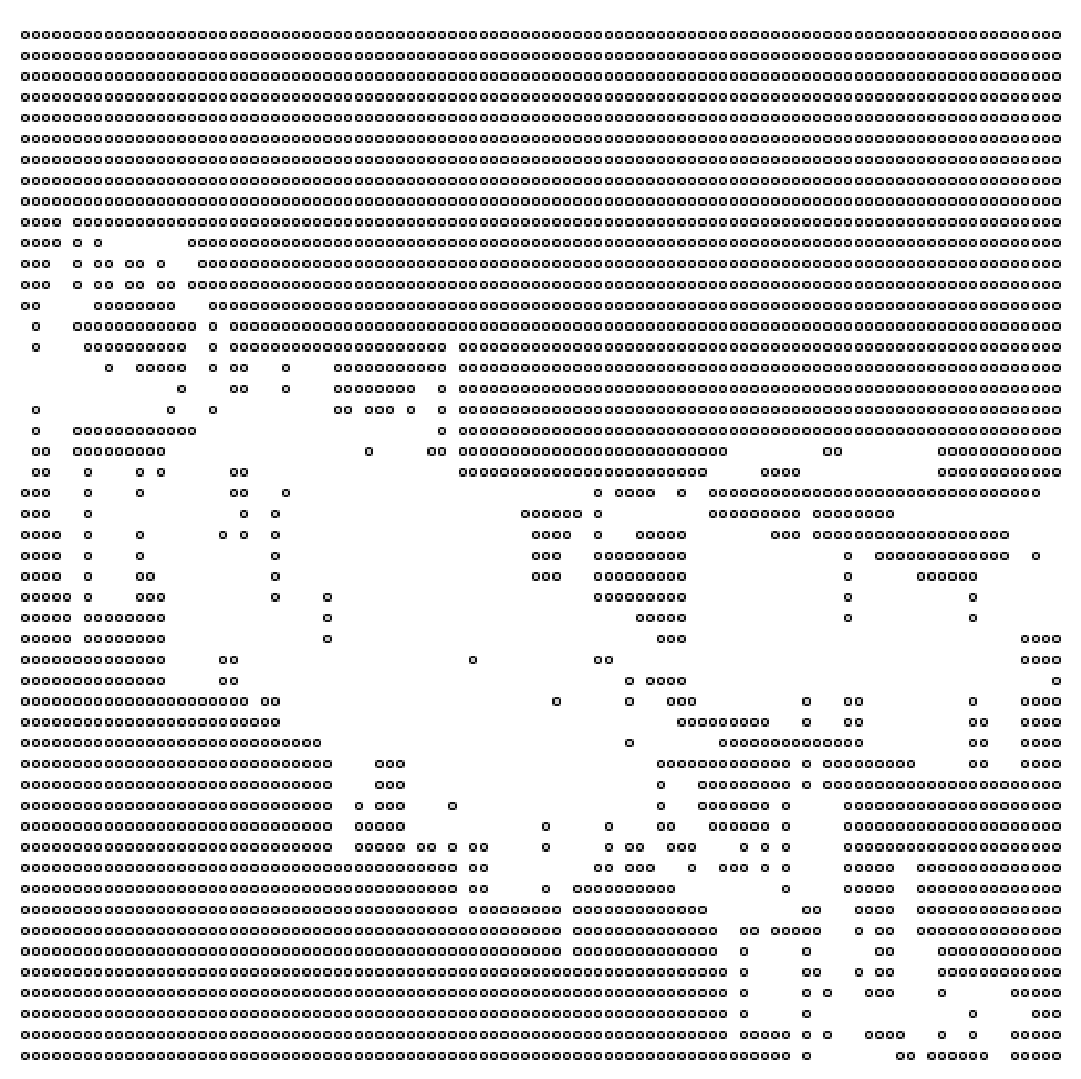
\includegraphics[totalheight=0.2\textheight,width=.6\textwidth]{mapa}
\caption {Vygenerovaná mapa}
\label{fig:mapa}
\end{figure}
